\chapter{Geometric Computations via Matrix-Free Linear Algebra}
\label{chap:linalg}



\begin{keypointsbox}
\noindent
\textbf{Key points (Chapter~\ref{chap:linalg}).}
\begin{enumerate}\setlength{\itemsep}{2pt}
  \item \textbf{The dataset-restricted model map.}
\end{enumerate}
\end{keypointsbox}

\begin{center}
\begin{minipage}{0.95\linewidth}
\noindent\textbf{Chapter \thechapter\ -- Geometric Computations via Matrix-Free Linear Algebra:}\par\vspace{3pt}

\begin{tabular}{@{}p{0.83\linewidth}r@{}}
\hyperref[sec:bridge_dg_la]{\thechapter.1\;\;From Geometry to Linear Algebra} \dotfill & \pageref{sec:bridge_dg_la}\\
\hyperref[sec:la_computations]{\thechapter.2\;\;Efficient Linear Algebra for Deep Learning} \dotfill & \pageref{sec:la_computations}\\
\end{tabular}
\end{minipage}
\end{center}


\noindent
In the previous chapter, we explored the parameter space geometry of models in Bayesian Deep Learning. However, to accomplish anything of practical significance, we need to be able to compute geometric quantities on this manifold. At first inspection, this task might seem completely hopeless. The parameter space is a $P$-dimensional manifold, where $P$ is the number of parameters, which can be at the order of billions. However, as we will show in this chapter, the decomposition of the tangent space of the manifold into the kernel and image can make various computations tractable. 

In this chapter, we will begin with a brief recap of the parameter space geometry derived from the previous chapter. We will then proceed to show how this geometry affects the computation of various geometric quantities that live on this manifold, and finally, how they mostly translate to well-known linear algebra problems. Finally, we will develop linear algebra algorithms that can scale to large models.

\section{From Geometry to Linear Algebra}
\label{sec:bridge_dg_la}

We will briefly summarise the parameter space geometry from the previous chapter, omitting the gnarly formal details, only assuming some familiarity with Riemannian Geometry \citep{Soren notes}. Let $\Theta$ denote the parameter space, typically $\Theta=\mathbb{R}^P$. We will show that in the Bayesian Deep Learning setting, a natural non-Euclidean geometry emerges on the parameter space. 

\subsection{Reparameterization and Overparameterization}
We can illustrate this nontrivial geometry with a simple example. Consider a function 
\begin{align}
    f_x(\theta) = \theta_2 \texttt{ReLu}(\theta_1 x)
\end{align}

where $ \texttt{ReLu}$ is the rectified linear unit function commonly used as an activation function in neural networks. $\texttt{ReLu}$ function is known to be invariant to scaling i.e. $\texttt{ReLu}(ax) = a \texttt{ReLu}(x)$. Thus for any $\alpha \neq 0$ we have that:
\begin{align}
     f_x(\theta) &= \theta_2 \texttt{ReLu}(\theta_1 x) \\
     &= \frac{\theta_2}{\alpha}\texttt{ReLu}(\alpha \theta_1 x)
\end{align}
For parameter vectors $\theta = (\theta_1, \theta_2)$ and $\hat{\theta} = (\frac{\theta_2}{\alpha}, \alpha \theta_1)$ the function $f_x$ generates the same predictions. This scaling transformation that maps $\theta$ to $\hat{\theta}$ is a \emph{reparameterization} of $f_x$, since despite being distinct parameters they generate identical outputs. This suggests that instead of treating the parameter space as a euclidean, we should endow it with a geometry that is aware of such reparameterizations. 

However, this is only an issue if such reparameterizations exist. This raises the question: Do neural networks always have such reparameterizations, and if so what are they? It is hard to explicitly enumerate \emph{all} reparameterizations of neural networks since they are dependent on the architecture and can become quite complex. 

We can address this problem by considering a broader class of reparameterizations that are both more informative in the Bayesian deep learning setting, guaranteed to exist under reasonable assumptions, and easier to characterise more or less exactly. Note that the scaling reparameterizations of the function $f_x(\theta)$ are completely independent of $x$, i.e., two parameters are equivalent if they generate the same output for all $x\in \mathbb{R}$. We will call such reparameterizations \emph{global reparameterizations}. Here we will consider a larger class of reparameterizations which we call \emph{data-dependent reparameterizations}.  

For a fixed dataset $\mathcal{D}= (x_1, \dots, x_N)$, we have a model map defined as $F_{\mathcal D}:\Theta\to \mathbb R^{NO}$ which maps each parameter to logits in the outputs space, $\theta \mapsto \eta = (\eta_1, \dots, \eta_N)$. These logits can then be used to compute the likelihood of the observed data. We say $\theta \sim \hat{\theta}$ if and only if they generate the same outputs for the fixed dataset $\mathcal D $ i.e., $F_{\mathcal D}(\theta) = F_{\mathcal D}(\hat{\theta)}$.

If $dim(\Theta) = P$ then, we say that the model map is \emph{overparameterized} if $P > NO$. Data-dependent reparameterizations are guaranteed to exist if the model map is overparameterized. We can see this by considering the Jacobian of the model map, $\mathbf{J}_\mathcal{D}(\theta) \in \mathbb{R}^{NO \times P}$. It defines a linear map between $\mathbb{R}^{NO}$ and $\mathbb{R}^P$. By the rank-nullity theorem, this linear map has a null-space, call it $\texttt{null}(\mathbf{J}_\mathcal{D}(\theta))$ of dimension $P - NO$. Any vector in this null space gives us directions in which we can infinitesimally perturb the parameters that do not change the outputs. Integrating along these directions will give us the data-dependent reparameterizations.

\subsection{Parameter Manifold}
Now that we have characterized reparameterizations of our model map, we will consider how this informs the geometry over the parameter space. We treat the parameter space $\Theta$ as a Riemannian manifold. At each $\theta$ we can split the tangent space into two different subspaces: $T_\theta\Theta = H_\theta \oplus V_\theta$, where $V_\theta = \texttt{null}(\mathbf{J}_\mathcal{D}(\theta))$ and $H_\theta = \texttt{im}(\mathbf{J}_\mathcal{D}(\theta)^\top)$ is its orthogonal complement. These correspond to reparameterization directions and directions that change predictions, respectively. 

The reason for making this decomposition of the tangent space is that we would like treat the notion of distance differently in these two subspaces. We define two smooth positive symmetric bilinear forms $g^{\mathrm{hor}}_\theta$ and $g^{\mathrm{ver}}_\theta$ on the Tangent subbundles (distributions) $H_\theta$ and $V_\theta$ respectively. These formalize the notion of length and angle of tangent vectors in these subspaces. We equip the parameter space with a Riemannian metric in the parameter space $g_\theta\;:=\; g^{\mathrm{hor}}_\theta \oplus \lambda\, g^{\mathrm{ver}}_\theta $, that is an orthogonal sum of two $g^{\mathrm{hor}}_\theta$ and $g^{\mathrm{ver}}_\theta$. For tangent vectors $(\delta,\varphi), \, (\delta', \varphi') \in T_\theta\Theta = H_\theta \oplus V_\theta$:

\begin{align}
    g_\theta((\delta,\varphi), (\delta', \varphi')) = g^{\mathrm{hor}}_\theta(\delta, \delta') + g^{\mathrm{ver}}_\theta(\varphi, \varphi')
\end{align}

This allows us to talk about distances on the parameter space, and we will return to this after a brief discussion of how to choose $g^{\mathrm{hor}}_\theta$ and $g^{\mathrm{ver}}$.
\paragraph{Prediction Space Distances}
To define a metric, $g^{\mathrm{hor}}_\theta$ on $H_\theta$, we recall that $H_\theta$ corresponds to tangent vectors which perturb our outputs. We can then choose a distance (more precisely, a Riemannian metric) on the output space and then pull back this metric to the parameter space to define $g^{\mathrm{hor}}_\theta$. This defines local distances between two parameters when they are perturbed by tangent vectors $H_\theta$ to be the corresponding perturbations in the outputs. If the metric on the output space is chosen to be $\mathbf{W}(\eta)$, then:
\begin{align}
    g^{\mathrm{hor}}_\theta(\delta, \delta') &= \langle \mathbf{J}_\mathcal{D}(\theta)\delta, \mathbf{J}_\mathcal{D}(\theta)\delta'   \rangle_{\mathbf{W}
    (\eta)} \\
    &= \delta^\top (\mathbf{J}_\mathcal{D}(\theta)^\top \mathbf{W}
    (\eta) \mathbf{J}_\mathcal{D}(\theta)) \delta'
\end{align}

Standard choices for $\mathbf{W}(\eta)$ include:
\begin{enumerate}
    \item \textbf{Euclidean Metric:} $\mathbf{W}
    (\eta) = \mathbb{I}$, which corresponds to pulling back the Euclidean distance from the output space to the parameter space and gives the Gauss-Newton metric on $H_\theta$, i.e.,$ g^{\mathrm{hor}}_\theta = \mathbf{J}_\mathcal{D}(\theta)^\top \mathbf{J}_\mathcal{D}(\theta)$.  
    \item \textbf{Fisher Information Metric:} $\mathbf{F}
    (\eta) = \mathbb{E}_{y\sim p(y|\eta)} [\nabla^2 \, \textrm{log}\, p(y|\eta)]$, where the expectation is typically approximated with a Monte-Carlo estimate over the dataset.  In the parameter space, this gives us the Fisher Information metric, i.e. $g^{\mathrm{hor}}_\theta = \mathbf{J}_\mathcal{D}(\theta)^\top \mathbf{F}
    (\eta)\mathbf{J}_\mathcal{D}(\theta)$.
    \item \textbf{Loss Hessian:} $\mathbf{H}
    (\eta) = \nabla^2_\eta \, \mathcal{L}_\mathcal{D}$, which corresponds to choosing the Bregman divergence as the distance in the output space. In the parameter space, this gives us the Generalized Gauss-Newton metric, i.e. $g^{\mathrm{hor}}_\theta = \mathbf{J}_\mathcal{D}(\theta)^\top \mathbf{H}
    (\eta)\mathbf{J}_\mathcal{D}(\theta)$. For standard deep learning likelihood functions, the Generalized Gauss-Newton coincides with the Fisher Information metric \citep{henning paper}.
\end{enumerate}
This metric must be restricted to $H_\theta$. To see this notice that for any choice of $\mathbf{W}(\eta)$ and the correponding pullback metric given by $g^{\mathrm{hor}}_\theta = \mathbf{J}_\mathcal{D}(\theta)^\top \mathbf{W}(\eta)\mathbf{J}_\mathcal{D}(\theta)$ has rank at most $NO$, even though $g^{\mathrm{hor}}_\theta$ is $P\times P$ matrix. This is because $\mathbf{J}_\mathcal{D}(\theta)$ is $NO \times P$ matrix. Thus, there are $P - NO$ directions in the tangent space that live in the null space of $g^{\mathrm{hor}}_\theta$. So choosing this metric on the entire tangent space, $T_\theta \Theta$, would lead to $g_\theta(u, v) = 0$, for any $u,v \in \texttt{null}(g^{\mathrm{hor}}_\theta)$. So $g_\theta$ would be a pseudo-metric which wouldn't properly account for reparameterizations, which has been our goal. 

\paragraph{Null Space Distance}
 To obtain a genuine Riemannian metric on $T_\theta\Theta$, we need to equip $V_\theta$ with a positive-definite quadratic form. Since perturbations in $H_\theta$ keep the outputs fixed, the metric on this subspace is independent of the predictions. The obvious choice is to choose a Euclidean metric (often scaled by the prior precision):
 \begin{align}
     g^{\mathrm{ver}}_\theta(\varphi,\varphi') := \alpha \varphi^\top \varphi
 \end{align}
 
 We can think of the geometry on the null-space as only capturing the properties of the prior, since it is independent of the likelihood. For a Gaussian prior with precision $\alpha$, this corresponds to the metric specified above. However, other choices of prior can lead to a different choice of metric on the null space directions, but for now, we will treat the scaled Euclidean metric as the canonical choice. 
 
After the discussion above, a natural question arises: \emph{Can we decompose the parameter space into image and kernel manifolds instead of only decomposing the tangent space?} We can prove that under mild assumptions, a kernel manifold exists consisting of parameters that generate the same outputs. This is a consequence of the well-known preimage theorem. However, the same cannot be said for the image manifold consisting of parameters that only generate distinct outputs. The existence of this manifold depends on the integrability of the subbundle $H_\theta$, which is characterised by the Frobenius theorem. It states that a subbundle is integrable (forms a submanifold) iff it is involutive. This condition is not satisfied in most cases. The image directions do not integrate to form a submanifold, except in very specific cases such as the linear gaussian example examined in \Cref{subsec:linear_gaussian_geometric_language}.
. 

\subsection{Translating Geometric Computations to Linear Algebra}
\label{subsec:geom_to_la}

Having defined the manifold structure of $\Theta$, we now address the practical computation of differential-geometric objects. We demonstrate that these complex quantities can be expressed in terms of three basic \emph{Linear Algebra Primitives}. We assume we have access to both the values and gradients of these primitives, i.e., we can efficiently solve these linear algebra problems and differentiate them wrt $\theta$.

\paragraph{Computational Primitives}
We assume access to the following operations, which will be implemented in later sections using matrix-free methods:

\begin{enumerate}
    \item \textbf{Primitive 1: Subspace Projections.}
    Given an arbitrary tangent vector $\mathbf{u} \in T_\theta \Theta$, we require the orthogonal projection onto the horizontal (prediction-affecting) and vertical (null) subspaces:
    \begin{align}
        \mathbf{u} &= \mathbf{u}_H + \mathbf{u}_V, \quad \text{where } \mathbf{u}_H \in H_\theta, \; \mathbf{u}_V \in V_\theta.
    \end{align}
    We denote these operations as $\mathbf{u}_H = \textsf{Proj}_H(\theta, \mathbf{u})$ and $\mathbf{u}_V = \textsf{Proj}_V(\theta, \mathbf{u})$.

    \item \textbf{Primitive 2: Least-squares solves}
    Given an arbitrary change $\mathbf{b} \in \mathbb{R}^{NO}$ in the output space, we define \textsf{Lstsq} as the least-squares problem:
    \begin{align}
    \label{eq:constr_lsq_param}
        \textsf{LstSq}(\theta, \mathbf{b}) \;&:=\;  \underset{\mathbf{v} \in T_\theta \Theta}{\arg\min} \, \|\mathbf{v}\|_2 \quad \text{s.t.} \quad \mathbf{W}(\eta)^{1/2}\mathbf{J}_\mathcal{D}(\theta)\mathbf{v} = \mathbf{b} \\
        &= \big(\mathbf{W}(\eta)^{1/2}\mathbf{J}_\mathcal{D}(\theta)\big)^\top \Big( \big(\mathbf{W}(\eta)^{1/2}\mathbf{J}_\mathcal{D}(\theta)\big) \big(\mathbf{W}(\eta)^{1/2}\mathbf{J}_\mathcal{D}(\theta)\big)^\top \Big)^{-1} \mathbf{b} \nonumber \\
        &= \mathbf{J}_\mathcal{D}(\theta)^\top \big(\mathbf{J}_\mathcal{D}(\theta)\mathbf{J}_\mathcal{D}(\theta)^\top\big)^{-1} \mathbf{W}(\eta)^{-1/2} \mathbf{b}. \nonumber
    \end{align}

    \item \textbf{Primitive 3: Spectral Functions (LogDet).}
    Finally, we assume we have access to log determinants of the metric:
    \begin{align}
        \textsf{LogDet}(\theta) \;:=\; \log\det\!\left(g^{\mathrm{hor}}_\theta|_{H_\theta}\right).
    \end{align}
\end{enumerate}

\paragraph{Decomposition of Metric Quantities}
Before deriving specific geometric quantities, we first characterize how the metric tensor and its inverse decompose under the orthogonal splitting of the tangent space $T_\theta \Theta = H_\theta \oplus V_\theta$. In a basis adapted to this split, the metric tensor $G(\theta)$ and its inverse $G(\theta)^{-1}$ are block-diagonal:

\begin{align}
    G(\theta) &= \begin{bmatrix} G_H(\theta) & 0 \\ 0 & G_V(\theta) \end{bmatrix} 
    = \begin{bmatrix} \mathbf{J}_\mathcal{D}(\theta)^\top \mathbf{W}(\eta) \mathbf{J}_\mathcal{D}(\theta) & 0 \\ 0 & \alpha \mathbb{I}_{P-N} \end{bmatrix}, \\
    G(\theta)^{-1} &= \begin{bmatrix} G_H(\theta)^{-1} & 0 \\ 0 & G_V(\theta)^{-1} \end{bmatrix} 
    = \begin{bmatrix} (\mathbf{J}_\mathcal{D}^\top \mathbf{W} \mathbf{J}_\mathcal{D})^\dagger & 0 \\ 0 & \frac{1}{\alpha} \mathbb{I}_{P-N} \end{bmatrix}.
\end{align}

Consequently, the log-determinant (volume density) also decomposes additively:
\begin{align}
    \log \det G(\theta) &= \log \det G_H(\theta) + \log \det G_V(\theta) \nonumber \\
    &= \textsf{LogDet}_H(\theta) + (P-N) \log \alpha.
\end{align}
This structure allows us to compute complex Riemannian quantities by treating the horizontal (data-dependent) and vertical (prior-dependent) components independently.

\paragraph{Geometric Quantities via Primitives}
We now express standard Riemannian quantities using this decomposition and the linear algebra primitives defined previously.

\begin{enumerate}
    \item \textbf{Riemannian Inner Product and Norm.}
    \emph{Concept:} The metric defines the fundamental notion of length and angle on the manifold.
    
    \emph{General Formula:} For tangent vectors $\mathbf{u}, \mathbf{v} \in T_\theta \Theta$, the inner product is $\langle \mathbf{u}, \mathbf{v} \rangle_G = \mathbf{u}^\top G(\theta) \mathbf{v}$.
    
    \emph{Decomposition:} Using the block-diagonal structure of $G$, this splits into:
    \begin{align}
        \langle \mathbf{u}, \mathbf{v} \rangle_G &= \mathbf{u}_H^\top G_H(\theta) \mathbf{v}_H + \mathbf{u}_V^\top G_V(\theta) \mathbf{v}_V
    \end{align}
    
    \emph{Approximation \& Primitives:} No approximation is required. We use \textbf{Primitive 1} to obtain the projections $\mathbf{u}_H, \mathbf{u}_V$, and then compute the quadratic forms:
    \begin{align}
        \|\mathbf{u}\|_G^2 &= \mathbf{u}_H^\top (\mathbf{J}^\top \mathbf{W} \mathbf{J}) \mathbf{u}_H + \alpha \|\mathbf{u}_V\|_2^2.
    \end{align}

    \item \textbf{Curve Length, Energy, and Geodesics.}
    \emph{Concept:} 
    The geometry of the parameter space allows us to measure the length of a continuous path $\gamma: [0,1] \to \Theta$ and its energy (or action). Geodesics are the "straight lines" of the manifold, defined as curves that locally minimize this energy functional.
    
    \emph{General Formula:}
    The length $\mathcal{L}(\gamma)$ and energy $E(\gamma)$ are defined by integrals of the Riemannian norm of the velocity vector $\dot{\gamma}(t)$:
    \begin{align}
        \mathcal{L}(\gamma) &= \int_0^1 \|\dot{\gamma}(t)\|_{g_{\gamma(t)}} \, dt \\
        E(\gamma) &= \frac{1}{2} \int_0^1 \|\dot{\gamma}(t)\|_{g_{\gamma(t)}}^2 \, dt.
    \end{align}
    Geodesics are curves that minimize the energy functional, satisfying the Euler-Lagrange equations $\delta E(\gamma) = 0$, corresponding to the shortest path between two points.
    
    \emph{Decomposition:}
    Using the orthogonal decomposition of the norm, the length and energy split into:
    \begin{align}
        & \mathcal{L}(\gamma) = \frac{1}{2} \int_0^1 \sqrt{\left( \|\dot{\gamma}(t)_H\|_{g^{\mathrm{hor}}}^2 + \alpha \|\dot{\gamma}(t)_V\|_2^2 \right)} \, dt \\
        &E(\gamma) = \frac{1}{2} \int_0^1 \left( \|\dot{\gamma}(t)_H\|_{g^{\mathrm{hor}}}^2 + \alpha \|\dot{\gamma}(t)_V\|_2^2 \right) \, dt.
    \end{align}
    
    \emph{Approximation \& Primitives:}
    \textbf{Length and Energy:}
    For a discretized path $\theta_{0:K}$, we approximate the integrals by summing the squared norms of the steps $\Delta \theta_k = \theta_{k+1} - \theta_k$. Using \textbf{Primitive 1} to decompose the step, the discrete length and energy is given by:
    \begin{align}
        &\mathcal{L}(\theta_{0:K}) \approx \frac{1}{2\Delta t} \sum_{k=0}^{K-1} \sqrt{ \big\| \textsf{Proj}_H(\theta_k, \Delta \theta_k) \big\|_{G^{\mathrm{hor}}}^2 + \alpha \big\| \textsf{Proj}_V(\theta_k, \Delta \theta_k) \big\|_2^2 }\\
        &E(\theta_{0:K}) \approx \frac{1}{2\Delta t} \sum_{k=0}^{K-1} \left( \big\| \textsf{Proj}_H(\theta_k, \Delta \theta_k) \big\|_{G^{\mathrm{hor}}}^2 + \alpha \big\| \textsf{Proj}_V(\theta_k, \Delta \theta_k) \big\|_2^2 \right).
    \end{align}
    
    \textbf{Geodesics (Variational Approach):}
    We approximate geodesics by minimizing the discrete energy $E(\theta_{0:K})$ with respect to the intermediate points $\theta_{1:K-1}$. This optimization requires the gradient $\nabla_{\theta_k} E$. 
    
    Critically, because the subspace splitting depends on the current parameter $\theta$, the gradient must differentiate through the projection operator. For the horizontal component $\mathbf{u}_H = \textsf{Proj}_H(\theta, \Delta \theta)$, the gradient is:
    \begin{align}
        \nabla_{\theta} \|\mathbf{u}_H\|_{G^{\mathrm{hor}}}^2 = 
        \underbrace{2 \big\langle \nabla_\theta \big( \textsf{Proj}_H(\theta, \Delta \theta) \big), \, \mathbf{u}_H \big\rangle_{G^{\mathrm{hor}}}}_{\text{Subspace Rotation}} 
        + \underbrace{\mathbf{u}_H^\top (\nabla_\theta G^{\mathrm{hor}}) \mathbf{u}_H}_{\text{Metric Change}}.
    \end{align}
    The term $\nabla_\theta \textsf{Proj}_H$ captures the non-integrability of the horizontal distribution (the "turning" of the tangent space), which is automatically computed via Automatic Differentiation of \textbf{Primitive 1}.    
    \item \textbf{Riemannian Gradient (Natural Gradient).}
    \emph{Concept:} The direction of steepest ascent on the manifold, adjusting the Euclidean gradient $\nabla_\theta \mathcal{L}$ for the local curvature.
    
    \emph{General Formula:} $\nabla^G \mathcal{L} = G(\theta)^{-1} \nabla_\theta \mathcal{L}$.
    
    \emph{Decomposition:} The inverse metric acts independently on the horizontal and vertical projections of the Euclidean gradient:
    \begin{align}
        \nabla^G \mathcal{L} &= G_H^{-1} (\nabla_\theta \mathcal{L})_H + G_V^{-1} (\nabla_\theta \mathcal{L})_V.
    \end{align}
    
    \emph{Approximation \& Primitives:} 
    For the horizontal component, we solve the linear system using \textbf{Primitive 2} (interpreting the gradient as a pullback $\mathbf{J}^\top \mathbf{g}_\eta$). For the vertical component, we simply scale by $1/\alpha$.
    \begin{align}
        (\nabla^G \mathcal{L})_H &\approx \textsf{LstSq}\big(\theta, \, \mathbf{W}^{-1/2} \nabla_\eta \mathcal{L}\big) \\
        (\nabla^G \mathcal{L})_V &= \frac{1}{\alpha} \textsf{Proj}_V\big(\theta, \, \nabla_\theta \mathcal{L}\big).
    \end{align}

    \item \textbf{Riemannian Volume Form.}
    \emph{Concept:} Measures the local density of the parameter space, essential for integration and computing the evidence.
    
    \emph{General Formula:} $\text{Vol}(\theta) = \sqrt{\det G(\theta)}$.
    
    \emph{Decomposition:} As noted in the introductory remarks, the determinant factorizes:
    \begin{align}
        \log \sqrt{\det G} = \frac{1}{2} \log \det G_H + \frac{1}{2} \log \det G_V.
    \end{align}
    
    \emph{Approximation \& Primitives:} The horizontal term is computed via \textbf{Primitive 3}. The vertical term is analytical.
    \begin{align}
        \log \sqrt{\det G} \approx \frac{1}{2} \textsf{LogDet}_H(\theta) + \frac{P-N}{2} \log \alpha.
    \end{align}

    \item \textbf{Laplace-Beltrami Operator.}
    \emph{Concept:} 
    The Laplacian $\Delta f$ is the divergence of the Riemannian gradient. It measures the local curvature of the function $f$ relative to the geometry of the manifold.
    
    \emph{General Formula:} 
    Expanding the divergence using the formula $\text{div}(\mathbf{X}) = \text{Tr}(\nabla_\theta \mathbf{X}) + \mathbf{X}^\top \nabla_\theta \log \sqrt{\det G}$, we obtain:
    \begin{align}
        \Delta f = \text{Tr}\big( \nabla_\theta (\nabla^G f) \big) + (\nabla^G f)^\top \nabla_\theta \log \sqrt{\det G}.
    \end{align}
    Note that $\nabla_\theta (\nabla^G f)$ is the standard Jacobian of the Riemannian gradient vector field.
    
    \emph{Decomposition:} 
    The vertical volume density is constant, so $\nabla_\theta \log \det G_V = 0$. The density correction comes purely from the horizontal component.
    \begin{align}
        \Delta f = \underbrace{\text{Tr}\big( \nabla_\theta (\nabla^G f) \big)}_{\text{Total Trace}} + \frac{1}{2} \underbrace{(\nabla^G f)_H^\top \nabla_\theta \big( \textsf{LogDet}_H(\theta) \big)}_{\text{Horizontal Density Correction}}.
    \end{align}
    
    \emph{Approximation \& Primitives:} 
    \textbf{Trace Term:} We estimate the trace using Hutchinson's estimator. We sample $\mathbf{z} \sim \mathcal{N}(0, I)$ and compute the directional derivative of the Riemannian gradient along $\mathbf{z}$.
    \begin{align}
        \text{Tr}\big( \nabla_\theta (\nabla^G f) \big) \approx \mathbb{E}_{\mathbf{z}} \left[ \mathbf{z}^\top \left( \partial_{\mathbf{z}} \big( \nabla^G f(\theta) \big) \right) \right].
    \end{align}
    Crucially, $\nabla^G f(\theta)$ is itself computed via our primitives (Item 2). The term $\partial_{\mathbf{z}} (\nabla^G f)$ is computed by AD differentiation \emph{through} the linear solve (\textbf{Primitive 2}) and projection (\textbf{Primitive 1}).
    
    \textbf{Density Term:} computed by differentiating \textbf{Primitive 3} (LogDet) and taking the dot product with the horizontal Riemannian gradient.

    \item \textbf{Levi-Civita Connection.}
    \emph{Concept:} 
    The connection $\nabla_{\mathbf{u}} \mathbf{v}$ generalizes the directional derivative to curved space. It corrects the standard Euclidean derivative $\partial_{\mathbf{u}} \mathbf{v}$ by adding a "turning" term (the Christoffel symbol $\Gamma(\mathbf{u}, \mathbf{v})$) that accounts for how the basis frames rotate as we move along $\mathbf{u}$.
    
    \emph{General Formula:} 
    For constant ambient vector fields $\mathbf{u}, \mathbf{v}$ (where $\partial_{\mathbf{u}}\mathbf{v} = 0$ and Lie brackets vanish), the connection is purely determined by the metric derivatives via the Koszul formula. For any test vector $\mathbf{w}$:
    \begin{align}
        2 \langle \nabla_{\mathbf{u}} \mathbf{v}, \mathbf{w} \rangle_G = \partial_{\mathbf{u}} \langle \mathbf{v}, \mathbf{w} \rangle_G + \partial_{\mathbf{v}} \langle \mathbf{u}, \mathbf{w} \rangle_G - \partial_{\mathbf{w}} \langle \mathbf{u}, \mathbf{v} \rangle_G.
    \end{align}
    This effectively defines $\nabla_{\mathbf{u}} \mathbf{v} = G^{-1} \mathbf{b}$, where $\mathbf{b}$ is the vector representing the R.H.S. linear functional in $\mathbf{w}$.
    
    \emph{Decomposition:} 
    Unlike the metric, the connection does not decompose into independent horizontal and vertical components because the subspaces themselves rotate (non-integrability). However, the computation of the result vector $\nabla_{\mathbf{u}} \mathbf{v}$ relies on the block-diagonal structure of the inverse metric $G^{-1}$ to invert the "force" vector $\mathbf{b}$.
    
    \emph{Approximation \& Primitives:} 
    We compute the vector $\mathbf{b}$ using Automatic Differentiation (AD) on the scalar metric terms, then apply the inverse metric:
    \begin{enumerate}
        \item \textbf{Compute Force Vector $\mathbf{b}$:} 
        Using AD, we compute the gradients corresponding to the three terms in the Koszul formula.
        \begin{align}
            \mathbf{b} = \frac{1}{2} \left( \nabla_\theta (\mathbf{v}^\top G \mathbf{u}) + \text{JVP}(\mathbf{u}, G\mathbf{v}) + \text{JVP}(\mathbf{v}, G\mathbf{u}) \right).
        \end{align}
        Here, $\text{JVP}(\mathbf{x}, G\mathbf{y})$ denotes the directional derivative $\partial_{\mathbf{x}}(G(\theta)\mathbf{y})$.
        \item \textbf{Apply Inverse Metric:}
        We solve for the connection vector by applying $G^{-1}$ to $\mathbf{b}$ using our primitives:
        \begin{align}
            \nabla_{\mathbf{u}} \mathbf{v} \approx \textsf{LstSq}\big(\theta, \mathbf{W}^{-1/2} \mathbf{J} \mathbf{b} \big) + \frac{1}{\alpha} \textsf{Proj}_V(\theta, \mathbf{b}).
        \end{align}
    \end{enumerate}    
\end{enumerate}

We have now seen that many key geometric quantities can be expressed in terms of three computational primitives described above. The rest of this chapter will consider the question of how to compute these primitives in a deep learning setting where we might have billions of parameters.

\section{Efficient Linear Algebra for Deep Learning}
\label{sec:la_computations}

\paragraph{The Philosophy of Differentiable Matrix-Free Linear Algebra}
In modern deep learning, we are typically \emph{memory constrained}: explicitly materializing large matrices and applying direct factorizations is often infeasible. For a model with $P$ parameters and a dataset of $N$ points with $O$ outputs, the Jacobian $\mathbf{J}_\mathcal{D}(\theta)$ contains $NOP$ elements. For modern architectures, where $P \approx 10^9$, explicitly instantiating such a matrix—let alone its $P \times P$ metric tensor—is strictly impossible due to memory constraints.
Crucially, however, we usually \emph{do} have efficient \emph{matrix--vector access} through the automatic differentiation engine: Jacobian-vector products (\textsf{JVP}) $\mathbf{v} \mapsto \mathbf{J}_{\mathcal D}(\theta)\mathbf{v}$ and vector-Jacobian products (\textsf{VJP}) $\mathbf{u} \mapsto \mathbf{J}_{\mathcal D}(\theta)^\top \mathbf{u}$ are standard building blocks in reverse/forward-mode AD and can be computed at a cost comparable to a (small constant multiple of) a forward/backward pass through the dataset.

The computational philosophy of this chapter is therefore to treat $\mathbf{J}_{\mathcal D}(\theta)$ (and related matrices such as $\mathbf{W}^{1/2}\mathbf{J}_{\mathcal D}(\theta)$) as \emph{linear operators} rather than matrix. Thus, we avoid direct methods such as Cholesky and LU decomposition that require instantiating the matrix. The geometric primitives from \Cref{subsec:geom_to_la} are then obtained using \emph{iterative} and \emph{matrix-free} methods---e.g.\ Krylov subspace methods, randomized estimators for traces/log-determinants ---all of which require only repeated applications of \textsf{JVP} and \textsf{VJP}. 

Finally, to make these primitives usable inside larger learning objectives, we require them to be differentiable with respect to $\theta$. Rather than backpropagating through every iteration of an algorithm (which is costly and numerically brittle), we differentiate \emph{implicitly} through the defining optimality conditions (or fixed-point equations) using adjoint/implicit differentiation. With a careful choice of formulation and constraints, the backward pass reduces to solving a linear system involving the \emph{same} operator as the forward computation (often reusing preconditioners and Krylov information), so that differentiation through these primitives can be implemented at a cost that is typically comparable to a single additional forward solve.

% \subsection{Primitive: Least-Squares Solves (\textsf{LstSq})}
% \label{subsec:lstsq_primitive}

% Many of our geometric computations reduce to solving a least-squares problem repeatedly, and doing so at deep-learning scale requires treating the solver as a \emph{matrix-free} and \emph{differentiable} operator.
% We therefore introduce the computational abstraction
% \begin{align}
% \label{eq:lstsq_operator_def}
% \mathbf{x}^\star \;=\; \texttt{LstSq}(\mathbf{A}(\theta), \mathbf{b}, \lambda),
% \end{align}
% which takes a linear operator $\mathbf{A}(\theta)$, a right-hand side $\mathbf{b}$, and a (possibly zero) regularisation parameter $\lambda$, and returns the corresponding least-squares solution.
% Throughout, $\mathbf{A}(\theta)$ is assumed too large to instantiate in memory and is accessed only through \emph{matvecs} and \emph{vecmats},
% \[
% (\theta,\mathbf{v}) \mapsto \mathbf{A}(\theta)\mathbf{v},
% \qquad
% (\theta,\mathbf{u}) \mapsto \mathbf{A}(\theta)^\top\mathbf{u}.
% \]

% \subsubsection{Values: Matrix-Free Least Squares}
% \label{subsubsec:lstsq_values}

% Let $m,n\in\mathbb{N}$, $\mathbf{b}\in\mathbb{R}^m$, and $\mathbf{A}(\theta)\in\mathbb{R}^{m\times n}$ be given.
% We distinguish \emph{tall} ($m\ge n$) from \emph{wide} ($m\le n$) systems, and \emph{regularised} from \emph{unregularised} systems depending on whether $\lambda\neq 0$.

% Concretely, \texttt{LstSq} solves
% \begin{subequations}
% \begin{align}
% \label{eq:lstsq_piecewise}
% \mathbf{x}^\star
% &=\texttt{LstSq}(\mathbf{A}(\theta),\mathbf{b},\lambda)
% \\
% &=
% \begin{cases}
% \arg\min_{\mathbf{x}}\;\|\mathbf{A}(\theta)\mathbf{x}-\mathbf{b}\|_2^2+\lambda^2\|\mathbf{x}\|_2^2,
% & \text{if }\lambda\neq 0\ \text{or }\mathbf{A}\text{ is tall},
% \\[3pt]
% \arg\min_{\mathbf{x}}\;\Big\{\|\mathbf{x}\|_2^2 \ \text{s.t.}\ \mathbf{A}(\theta)\mathbf{x}=\mathbf{b}\Big\},
% & \text{if }\lambda=0\ \text{and }\mathbf{A}\text{ is wide}.
% \end{cases}
% \end{align}
% \end{subequations}
% For tall $\mathbf{A}(\theta)$, the regularised formulation remains well-defined as $\lambda\to 0$ (in the sense of admitting a unique limit).
% For wide $\mathbf{A}(\theta)$, the unregularised case is instead defined explicitly as the minimum-norm solution of the underdetermined system.

% When $\lambda\neq 0$, the solution admits the equivalent representations
% \begin{subequations}
% \begin{align}
% \label{eq:lstsq_closed_form}
% \mathbf{x}^\star(\theta,\mathbf{b},\lambda)
% &=\mathbf{A}(\theta)^\top\!\big(\mathbf{A}(\theta)\mathbf{A}(\theta)^\top+\lambda^2\mathbf{I}\big)^{-1}\mathbf{b},
% \\
% &=\big(\mathbf{A}(\theta)^\top\mathbf{A}(\theta)+\lambda^2\mathbf{I}\big)^{-1}\mathbf{A}(\theta)^\top\mathbf{b}.
% \end{align}
% \end{subequations}
% In the limit $\lambda\to 0$, only one of these parameterisations is well-defined depending on whether $\mathbf{A}(\theta)$ is tall or wide.

% \paragraph{Why matrix-free, and why not normal equations.}
% Least-squares solvers can be broadly classified along two axes:
% (i) \emph{direct} versus \emph{matrix-free} methods (instantiate $\mathbf{A}$ versus access only via matvecs/vecmats),
% and (ii) solvers based on the linear systems in \eqref{eq:lstsq_closed_form} (``normal-equation style'') versus solvers based on \emph{orthogonal transformations}.
% Normal-equation style methods apply $\mathbf{v}\mapsto(\mathbf{A}^\top\mathbf{A}+\lambda^2\mathbf{I})^{-1}\mathbf{v}$ (or its wide analogue), which squares the singular values of $\mathbf{A}$ and therefore exacerbates conditioning, often requiring higher precision and slowing down iterative convergence.

% \paragraph{Bidiagonalisation and LSMR.}
% A numerically robust alternative is to avoid squaring altogether by using Golub--Kahan bidiagonalisation, which underlies LSQR and LSMR.
% These methods build a small bidiagonal surrogate of $\mathbf{A}$ using only matvecs and vecmats, and extract an approximate solution without forming $\mathbf{A}^\top\mathbf{A}$ or $\mathbf{A}\mathbf{A}^\top$.
% Crucially, there exist error-adaptive implementations with $\mathcal{O}(\max\{m,n\})$ memory.
% In our implementation of \texttt{LstSq}, we use \textbf{LSMR}, which is mathematically equivalent to applying MINRES to the regularised normal equations, but is typically more robust in practice because it treats $\mathbf{A}$ and $\mathbf{A}^\top$ separately rather than in combination (thus avoiding an explicit ``squaring'' step).

% \paragraph{Automatic transpose via autodiff.}
% Iterative bidiagonalisation solvers require both $\mathbf{A}(\theta)\mathbf{v}$ and $\mathbf{A}(\theta)^\top\mathbf{u}$.
% Manually implementing the transpose operator is error-prone, especially when $\mathbf{A}(\theta)$ is itself defined implicitly by a program.
% Instead, we obtain $\mathbf{A}(\theta)^\top$ automatically from a single vector-Jacobian product (VJP) on the (known-linear) forward map:
% \begin{align}
% \label{eq:auto_transpose_vjp}
% \Big[\mathbf{A}(\theta)\mathbf{v}_0,\;\big(\mathbf{u}\mapsto \mathbf{A}(\theta)^\top\mathbf{u}\big)\Big]
% \;=\;
% \texttt{vjp}\!\left(\mathbf{v}\mapsto \mathbf{A}(\theta)\mathbf{v},\ \mathbf{v}_0\right).
% \end{align}
% Thus, the solver only needs access to the forward linear operator $\mathbf{v}\mapsto \mathbf{A}(\theta)\mathbf{v}$; the transposed operator emerges from autodiff with minimal overhead.

% \subsubsection{Gradients: Adjoint Differentiation of \texttt{LstSq}}
% \label{subsubsec:lstsq_gradients}

% To use \texttt{LstSq} inside larger learning pipelines, we must differentiate through the solution map
% \(
% (\theta,\mathbf{b},\lambda)\mapsto \mathbf{x}^\star(\theta,\mathbf{b},\lambda).
% \)
% A naive approach is to \emph{backpropagate through the solver iterations} by unrolling LSMR.
% This is often slow and memory-intensive, since reverse-mode differentiation must traverse (and typically store) the entire iterative trajectory.

% Instead, we treat \texttt{LstSq} as an \emph{implicit layer} and derive custom reverse-mode derivatives using the \emph{adjoint method}.
% This yields a backward pass that requires only a small number of additional least-squares solves, and---with a matched tolerance---has essentially the same asymptotic cost profile as the forward pass (up to a small constant factor).

% \paragraph{Setup.}
% Let $\mu=\mu(\mathbf{x}^\star)$ be a scalar downstream objective and assume we are given $\nabla_{\mathbf{x}}\mu$.
% We seek $\nabla_\theta\mu$, $\nabla_{\mathbf{b}}\mu$, and $\nabla_\lambda\mu$ without ever forming $\nabla_{\mathbf{A}}\mu$ (which would be as large as $\mathbf{A}$ itself).
% The result below states custom reverse-mode rules in terms of additional calls to \texttt{LstSq}.

% \begin{theorem}[Reverse-mode derivatives of \texttt{LstSq}]
% \label{thm:lstsq_vjp}
% Let $\mathbf{A}(\theta)$ be full-rank and accessed only through matvecs/vecmats.
% Let $\mathbf{x}^\star=\texttt{LstSq}(\mathbf{A}(\theta),\mathbf{b},\lambda)$ and $\mu=\mu(\mathbf{x}^\star)$.
% Then the following hold.

% \begin{enumerate}
% \item \textbf{Tall case.}
% Suppose $\mathbf{A}(\theta)$ is tall and $\mathbf{x}^\star$ solves the (possibly damped) problem in \eqref{eq:lstsq_piecewise}.
% Define the residual $\mathbf{r}\coloneqq \mathbf{A}(\theta)\mathbf{x}^\star-\mathbf{b}$ and the auxiliary solve
% \[
% \boldsymbol{\xi}\;\coloneqq\;\texttt{LstSq}\!\big(\mathbf{A}(\theta),\,\nabla_{\mathbf{b}}\mu,\,0\big).
% \]
% Then
% \begin{subequations}
% \begin{align}
% \nabla_{\mathbf{b}}\mu
% &=\texttt{LstSq}\!\big(\mathbf{A}(\theta)^\top,\ \nabla_{\mathbf{x}}\mu,\ \lambda\big),
% \\
% \nabla_{\lambda}\mu
% &=2\lambda\,\langle \boldsymbol{\xi},\mathbf{x}^\star\rangle,
% \\
% \nabla_{\theta}\mu
% &=\nabla_{\theta}g(\theta),
% \qquad
% g(\theta)\coloneqq \langle \mathbf{r},\mathbf{A}(\theta)\boldsymbol{\xi}\rangle
% +\langle \nabla_{\mathbf{b}}\mu,\mathbf{A}(\theta)\mathbf{x}^\star\rangle.
% \end{align}
% \end{subequations}

% \item \textbf{Wide case.}
% Suppose $\mathbf{A}(\theta)$ is wide and $\mathbf{x}^\star$ solves the wide formulation in \eqref{eq:lstsq_piecewise} (or its damped variant).
% Define the residual
% \[
% \mathbf{r}\;\coloneqq\;\mathbf{A}(\theta)^\top\nabla_{\mathbf{b}}\mu-\nabla_{\mathbf{x}}\mu,
% \]
% and the auxiliary solve
% \[
% \mathbf{y}\;\coloneqq\;\texttt{LstSq}\!\big(\mathbf{A}(\theta)^\top,\ \mathbf{x}^\star,\ 0\big).
% \]
% Then
% \begin{subequations}
% \begin{align}
% \nabla_{\mathbf{b}}\mu
% &=\texttt{LstSq}\!\big(\mathbf{A}(\theta)^\top,\ \nabla_{\mathbf{x}}\mu,\ \lambda\big),
% \\
% \nabla_{\lambda}\mu
% &=-2\lambda\,\langle \nabla_{\mathbf{b}}\mu,\mathbf{y}\rangle,
% \\
% \nabla_{\theta}\mu
% &=\nabla_{\theta}g(\theta),
% \qquad
% g(\theta)\coloneqq \langle \nabla_{\mathbf{b}}\mu,\mathbf{A}(\theta)\mathbf{x}^\star\rangle
% +\langle \mathbf{y},\mathbf{A}(\theta)\mathbf{r}\rangle.
% \end{align}
% \end{subequations}
% \end{enumerate}
% \end{theorem}

% \paragraph{Backprop-through-iterations vs.\ implicit/adjoint differentiation.}
% The practical takeaway of \Cref{thm:lstsq_vjp} is that the backward pass through an adaptive matrix-free least-squares solver can be implemented without unrolling the solver loop.
% Instead, the reverse pass reduces to a small number of additional least-squares calls on $\mathbf{A}(\theta)$ or $\mathbf{A}(\theta)^\top$ (plus standard automatic differentiation of scalar functions like $g(\theta)$ that call matvecs/vecmats).
% Empirically, this adjoint-based VJP is substantially faster than differentiating by unrolling an iterative solver, while introducing only approximation error commensurate with the solver tolerance (since the backward pass is itself composed of least-squares solves on related systems).

% \paragraph{Remark (rank-deficient systems).}
% If $\mathbf{A}(\theta)$ is rank-deficient, the undamped tall problem is not uniquely solvable and therefore not differentiable without additional branch-selection.
% With nonzero damping ($\lambda\neq 0$), the solution becomes unique and the adjoint strategy extends with minor modifications by expressing the required adjoints through nested least-squares calls and null-space projections.

\section{Primitive: Matrix-Free Least-Squares (\textsf{LstSq})}
\label{sec:lstsq_primitive}

A central computational primitive in our framework is the method of least squares. We introduce a computational abstraction \textsf{LstSq}, which takes a linear operator $\mathbf{A}$, a vector $\mathbf{b}$, and a (potentially zero) regularization weight $\lambda$, and returns the optimal solution $\mathbf{x}^\star$.

\subsection{Values: Bidiagonalization and LSMR}

For any $m, n \in \mathbb{N}$, let $\mathbf{b} \in \mathbb{R}^m$ and $\mathbf{A} \in \mathbb{R}^{m \times n}$ be given. We assume the matrix $\mathbf{A}$ has full rank and is parameterized by some $\theta$, such that $\mathbf{A} = \mathbf{A}(\theta)$. Concretely, the \textsf{LstSq} method solves:
\begin{align}
\label{eq:constr_lsq_param}
    \mathbf{x}^\star 
    &= \textsf{LstSq}(\mathbf{A}(\theta), \mathbf{b}, \lambda)
    &= \begin{cases} 
    \arg\min_{\mathbf{x}} \|\mathbf{A}(\theta) \mathbf{x} - \mathbf{b}\|^2  + \lambda^2 \|\mathbf{x}\|^2 
    \quad \text{if}~\lambda \neq 0 \text{ or $\mathbf{A}$ is tall}, \\ 
    \arg\min_{\mathbf{x}}\left\{ \|\mathbf{x}\|^2 ~ \text{s.t.} ~ \mathbf{A}(\theta) \mathbf{x} = \mathbf{b} \right\} 
    \quad \text{if $\lambda = 0$\text{ and }$\mathbf{A}$ is wide.}
    \end{cases} \nonumber
\end{align}

The various methods for numerically solving least squares problems can be broadly classified across two axes.
Along one axis, there are \emph{direct} versus \emph{matrix-free} methods, which differ in whether or not the matrix $\mathbf{A}(\theta)$ is instantiated in memory (``direct method'', high memory demands, and for deep-learning-sized problems, $\mathbf{A}(\theta)$ is too big to store in memory) or only accessed via matrix-vector products (``matrix-free methods'', low memory demands).
Along the other axis, there are approaches based on solving the linear system in \Cref{equation-least-squares-solution-regularized} versus those approaches that apply orthogonal transformations to $\mathbf{A}(\theta)$ and extract $\mathbf{x}^\star$ directly, for example, using Golub-Kahan-Li bidiagonalization \citep{golub1965calculating}. 

Methods relying on the normal equations, such as Conjugate Gradient (CG), suffer a critical drawback: squaring the matrix $\mathbf{A}$ exacerbates ill-conditioning, as the eigenvalues of $\mathbf{A}^\top \mathbf{A}$ are the squared singular values of $\mathbf{A}$. As demonstrated in ~\Cref{figure:bidiag-vs-cg}, bidiagonalization-based solvers maintain numerical reliability even as the condition number approaches machine precision. Only matrix-free methods that target orthogonal transformations combine low memory demands with the ability to work in low precision, which is why we focus on this class of solvers. 

\begin{table}[h]
\centering
\caption{\textbf{Approaches to solving least squares.} ``L.S.'': linear system; ``O.T.'': orthogonal transformation.}
\label{tab:summary_of_methods}
\small
\begin{tabular}{llcc}
\toprule
\textbf{Method}& \textbf{Property} & \textbf{Direct} & \textbf{Matrix-free} \\
\midrule
\multirow{3}{*}{ \textbf{L.S.}} 
& Examples & Cholesky & Conj. Grad. \\
& Precision & Double  & Double \\
& Memory       & $\mathcal{O}(\min(m,n)^2)$ &$ \mathcal{O}(\max\{m, n\})$ \\
\midrule
\multirow{3}{*}{ \textbf{O.T.}} 
& Examples & SVD, QR &  LSMR \\
& Precision & {Single} & Single \\
& Memory      & $\mathcal{O}(mn)$ & $ \mathcal{O}(\max\{m, n\})$ \\
\bottomrule
\end{tabular}
\end{table}

\newcommand{\BidiagCGTheme}{Bidiagonalization vs. CG}
\begin{example}[\BidiagCGTheme{}]
\label{example-bidiag-vs-cg}
Consider the following least-squares problem: $A$ is a randomly populated $10^5 \times 50$ matrix with singular values in 
$[1, 1/\epsilon]$ where $\epsilon$ is machine precision ($\approx 10^{-7}$).
Least-squares based on bidiagonalisation is closely related to solving the normal equations with CG \citep{paige1982lsqr}, but the fact that solving the normal equation via CG requires $\mathbf{A} \mathbf{A}^\top$, whereas bidiagonalization handles $\mathbf{A}$, affects the numerical reliability of the algorithm; see \Cref{figure:bidiag-vs-cg}.
For well-conditioned matrices, the choice between CG and bidiagonalization would not matter much. But for ill-conditioned matrices, where numerical robustness is important, solving least squares problems with bidiagonalization instead of CG is vital.
\end{example}
% FIGURE 1
\begin{wrapfigure}{l}{0.38\columnwidth}
\centering
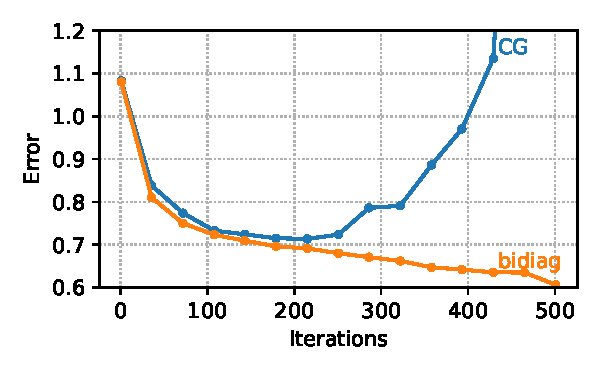
\includegraphics[width=0.95\linewidth]{chapters/ch4_figures/bidiag-vs-cg.pdf}
\caption{\BidiagCGTheme{}.}
\label{figure:bidiag-vs-cg}
\end{wrapfigure}


Specifically, we implement the \textsf{LstSq} primitive using \textbf{LSMR} \citep{fong2011lsmr}. This algorithm belongs to the family of \textbf{Krylov subspace methods}, which seek to approximate the solution to a high-dimensional linear problem within a subspace spanned by repeated applications of the operator on the initial residual: $\mathcal{K}_k(\mathbf{A}^\top\mathbf{A}, \mathbf{A}^\top\mathbf{b}) = \text{span}\{\mathbf{r}_0, (\mathbf{A}^\top\mathbf{A})\mathbf{r}_0, \dots, (\mathbf{A}^\top\mathbf{A})^{k-1}\mathbf{r}_0\}$. In these methods, the large, complex operator is decomposed into a product of orthogonal bases and a simplified, structured matrix (typically tridiagonal or bidiagonal), allowing the core optimization problem to be solved efficiently in a reduced-dimensional space.

To avoid the numerical instability of squaring the condition number inherent in the normal equations, we utilize the \textbf{Golub-Kahan Bidiagonalization (GKB)} \citep{golub1965calculating}. GKB is the natural extension of Krylov methods to rectangular matrices, iteratively generating two matrices with orthonormal columns, $\mathbf{U} \in \mathbb{R}^{m \times k}$ and $\mathbf{V} \in \mathbb{R}^{n \times k}$, and a lower bidiagonal matrix $\mathbf{B} \in \mathbb{R}^{k \times k}$ such that:
\begin{align}
\mathbf{A} \mathbf{V}_k = \mathbf{U}_{k+1} \mathbf{B}_k, \quad \mathbf{A}^\top \mathbf{U}_{k+1} = \mathbf{V}_k \mathbf{B}_k^\top + \alpha_{k+1} \mathbf{v}_{k+1} \mathbf{e}_{k+1}^\top.
\end{align}



This decomposition allows the high-dimensional least-squares problem to be projected onto the bidiagonal matrix $\mathbf{B}$, where the solution $\mathbf{x}^\star$ is approximated as:
\begin{align}\label{equation-bidiagonalization-for-lstsq}
\mathbf{x}^\star \approx \|\mathbf{b}\| \mathbf{V} (\mathbf{B}^\top)^{-1} \mathbf{e}_1.
\end{align}
While a naive implementation of GKB would require storing the full orthogonal bases $\mathbf{U}$ and $\mathbf{V}$—a feat impossible at deep learning scales—\textbf{LSMR} utilizes a clever short-recurrence formulation. This enables an error-adaptive, $\mathcal{O}(\max\{m, n\})$-memory solver that reaches the desired precision without ever explicitly storing or instantiating the orthogonal matrices, making it the ideal candidate for matrix-free geometric computations.\subsection{Gradients: Adjoint of the Least-Squares Problem}

If the solution $\mathbf{x}^\star$ is passed to a downstream loss $\mu(\mathbf{x}^\star)$, we require the backward pass through \textsf{LstSq} to optimize $\mu$ with respect to $\theta, \mathbf{b}$, or $\lambda$. 

\begin{theorem}[Gradients of \textsf{LstSq}]
\label{theorem:lsq_gradients}
Let $\mathbf{A}(\theta)$ be a full-rank matrix and $\lambda \in \mathbb{R}$ a regularisation weight. For a scalar objective $\mu(\mathbf{x}^\star)$, the following hold:
\begin{enumerate}
\item \textbf{Tall Case:}
$\nabla_{\mathbf{b}}\mu = \textsf{LstSq}(\mathbf{A}^\top,\nabla_{\mathbf{x}}\mu, \lambda)$ and $\nabla_{\theta} \mu = \nabla_{\theta} (\langle \mathbf{r}, \mathbf{A} \xi \rangle + \langle \nabla_{\mathbf{b}} \mu, \mathbf{A} \mathbf{x}^\star \rangle)$.
\item \textbf{Wide Case:}
$\nabla_{\mathbf{b}}\mu = \textsf{LstSq}(\mathbf{A}^\top, \nabla_{\mathbf{x}}\mu, \lambda)$ and $\nabla_{\theta} \mu = \nabla_{\theta}(\langle \nabla_{\mathbf{b}} \mu, \mathbf{A} \mathbf{x} \rangle + \langle \mathbf{y}, \mathbf{A} \mathbf{r} \rangle)$.
\end{enumerate}
\end{theorem}

\paragraph{Efficiency of Custom Gradients}
The primary advantage of these custom adjoints is computational efficiency. As shown in Figure~\ref{figure:adjoint-vs-ad}, our custom vector-Jacobian product (VJP) implementation is five to ten times faster than automatic differentiation performed by unrolling the solver's internal loop. 


\label{figure:adjoint-vs-ad}

This performance gap stems from the fact that the adjoint method requires exactly two additional forward-like passes (one for $\nabla_{\mathbf{b}}$ and one for $\xi$ or $\mathbf{y}$), whereas unrolling the solver requires storing and differentiating through every intermediate bidiagonalization step. Furthermore, Table~\ref{tab:precision-experiment} confirms that the gradient error remains proportional to the solver's forward tolerance, justifying the use of identical precision for both passes.

\section{Primitive: Subspace Projections (\textsf{Proj})}
\label{sec:subspace_projections}

The second primitive requires the orthogonal projection of an arbitrary tangent vector $\mathbf{u} \in T_\theta \Theta$ onto the horizontal (prediction-affecting) and vertical (null) subspaces.
\begin{align}
    \mathbf{u} &= \textsf{Proj}_H(\theta, \mathbf{u}) + \textsf{Proj}_V(\theta, \mathbf{u}) \\
    \text{where} \quad \textsf{Proj}_H(\theta, \mathbf{u}) &\in \text{im}(\mathbf{J}_\mathcal{D}(\theta)^\top) \quad \text{and} \quad \textsf{Proj}_V(\theta, \mathbf{u}) \in \text{ker}(\mathbf{J}_\mathcal{D}(\theta)).
\end{align}
While the \textsf{LstSq} primitive discussed previously can theoretically compute these projections, direct methods fail to exploit the specific row-partitioned structure of neural network Jacobians, which is crucial for scalability.

\subsection{Values: Alternating Projections}
We define the horizontal projection using the standard formula for the projection onto the row-space of $\mathbf{J}$:
\begin{equation}
    \label{eq:projection_basic_expression}
    \textsf{Proj}_H(\theta, \mathbf{u}) = \mathbf{J}^\top (\mathbf{J}\mathbf{J}^\top)^{-1} \mathbf{J} \mathbf{u}.
\end{equation}
Computing this directly requires inverting the $NO \times NO$ matrix $\mathbf{J}\mathbf{J}^\top$, which is infeasible. Instead, we focus on the vertical projection $\textsf{Proj}_V = \mathbb{I} - \textsf{Proj}_H$. We observe that the kernel of $\mathbf{J}$ is the intersection of the kernels of its row-partitions (batches):
\begin{align}
\label{eq: sum_ker}
  \text{ker}(\mathbf{J}) = \text{ker}\left(\sum_b \mathbf{J}_b^\top \mathbf{J}_b\right) = \bigcap_b \text{ker}(\mathbf{J}_b^\top \mathbf{J}_b).
\end{align}
To compute the projection onto this intersection, we employ \citeauthor{Neumann1949OnRO}'s method of \textbf{alternating projections}. As illustrated in Figure~\ref{fig:altproj}, projecting cyclically onto the individual null-spaces of each batch converges to the projection onto their intersection.


\begin{figure}[h]
    \centering
    \caption{To project a point onto the intersection of two subspaces, we alternate between projecting onto the individual subspaces.}
    \label{fig:altproj}
\end{figure}

Formally, we state the convergence of the vertical projection using the alternating projections method as follows:

\begin{theorem}[Alternating Projections for Subspace Intersection]
    \label{thm:altproj_convergence}
    Let the Jacobian $\mathbf{J}$ be partitioned into $B$ row-blocks, such that the kernel of the full Jacobian is the intersection of the per-block kernels, $\text{ker}(\mathbf{J}) = \bigcap_{b=1}^B \text{ker}(\mathbf{J}_b)$. The projection onto the vertical subspace $\textsf{Proj}_V(\theta, \mathbf{u})$ is given by the limit of the sequence:
    \begin{equation}
      \label{eq:altproj}
        \textsf{Proj}_V(\theta, \mathbf{u}) = \lim_{t\rightarrow\infty}
        \left(
          \prod_{b=1}^B
            \left(
                \mathbb{I} - \textsf{Proj}_{H_b}(\theta, \cdot)
            \right)
        \right)^t \mathbf{u},
    \end{equation}
    where $\textsf{Proj}_{H_b}(\theta, \cdot)$ denotes the orthogonal projection onto the row-space of the $b$-th batch Jacobian $\mathbf{J}_b$. The sequence converges linearly with a rate bounded by $c = \prod_{b=1}^{B-1} \cos^2(\theta_b)$, where $\theta_b$ is the minimum principal angle between the subspace of block $b$ and the intersection of the subspaces of the remaining blocks $j > b$.
\end{theorem}
\paragraph{Implementation: Block-wise Inversion.}
The efficiency of this method relies on the block-wise projections. For a small batch size $S$, $\textsf{Proj}_{H_b}$ requires inverting only an $SO \times SO$ matrix $\mathbf{J}_b \mathbf{J}_b^\top$. As shown in Figure~\ref{fig:projection_matrices}, this replaces one massive inversion with a sequence of small, manageable operations.


\begin{figure}[h]
    \centering
    \caption{\textbf{Visualization of Jacobian projections.} Direct calculation (left) involves inverting a large matrix. This is replaced by a series of cheap projections (right) using small $SO \times SO$ inverses.}
    \label{fig:projection_matrices}
\end{figure}

For well-conditioned blocks, we compute these small inverses using \textbf{direct methods} (e.g., Cholesky factorization) and cache the factors for reuse across the $t$ iterations. However, the blocks $\mathbf{J}_b$ happen to be ill-conditioned, we can substitute the direct inverse with an iterative \textsf{LstSq} solve (LSMR) for that specific block, ensuring numerical stability without compromising the overall algorithm.

\subsection{Gradients: Differentiable Projections via \textsf{LstSq}}
Differentiation through the unrolled alternating projection loop is memory-intensive and numerically drift-prone. Instead, we derive exact gradients by expressing the projection primitive in terms of the \textsf{LstSq} primitive.
We observe that the horizontal projection is exactly the solution to a specific least-squares problem mapped back to the tangent space:
\begin{align}
    \textsf{Proj}_H(\theta, \mathbf{u}) &= \mathbf{J}^\top \mathbf{x}^\star, \\
    \text{where} \quad \mathbf{x}^\star &= \textsf{LstSq}(\mathbf{J}^\top, \mathbf{u}, 0).
\end{align}
Here, $\textsf{LstSq}(\mathbf{J}^\top, \mathbf{u}, 0)$ computes $(\mathbf{J}\mathbf{J}^\top)^{-1}\mathbf{J}\mathbf{u}$ (in the wide case). Consequently, the gradients of $\textsf{Proj}_H$ (and by extension $\textsf{Proj}_V$) with respect to $\theta$ are fully defined by \cref{theorem:lsq_gradients}. This allows us to compute sensitivities of geometric projections efficiently using the adjoint method, treating the alternating projection solver as a black-box oracle for the forward pass.

\section{Primitive: Spectral Functions (\textsf{LogDet})}
\label{sec:logdet_primitive}

The final primitive required for our geometric computations is the evaluation of spectral functions, specifically the log-determinant of the generalized Gauss-Newton matrix $\mathbf{G}(\theta)$. This quantity is critical for the Riemannian volume form (to normalize the posterior) and the Laplace-Beltrami operator (to correct for curvature).

\subsection{Values: Stochastic Lanczos Quadrature}

Directly computing $\log\det \mathbf{G}(\theta)$ requires cubic time $\mathcal{O}(P^3)$ and quadratic memory $\mathcal{O}(P^2)$, which is infeasible for modern neural networks where $P \approx 10^7-10^9$. To approximate this, we combine the identity $\log\det \mathbf{A} = \text{tr}(\log \mathbf{A})$ with \textbf{Stochastic Trace Estimation (STE)} \citep{1989hutchinson}:
\begin{align}
    \textsf{LogDet}(\theta) &= \text{tr}(\log \mathbf{G}(\theta)) \nonumber \\
    &\approx \frac{1}{L} \sum_{l=1}^L \mathbf{v}_l^\top \log(\mathbf{G}(\theta)) \mathbf{v}_l, \quad \text{where } \mathbf{v}_l \sim \mathcal{N}(0, \mathbf{I}).
\end{align}
Evaluating the matrix-function-vector product $\log(\mathbf{G}(\theta))\mathbf{v}_l$ remains non-trivial. For this, we employ the \textbf{Lanczos iteration}, a Krylov subspace method for symmetric matrices. Given a starting vector $\mathbf{v}$, the Lanczos iteration decomposes the large operator $\mathbf{G}$ into a product involving an orthogonal matrix $\mathbf{Q}_K \in \mathbb{R}^{P \times K}$ and a small symmetric tridiagonal matrix $\mathbf{T}_K \in \mathbb{R}^{K \times K}$ such that $\mathbf{G} \approx \mathbf{Q}_K \mathbf{T}_K \mathbf{Q}_K^\top$.



Crucially, the columns of $\mathbf{Q}_K$ form an orthonormal basis for the Krylov subspace $\mathcal{K}_K(\mathbf{G}, \mathbf{v})$. We can then approximate the quadratic form by projecting the function onto this subspace:
\begin{align}
    \mathbf{v}^\top \log(\mathbf{G}) \mathbf{v} 
    &\approx \mathbf{v}^\top \mathbf{Q}_K \log(\mathbf{T}_K) \mathbf{Q}_K^\top \mathbf{v} \nonumber \\
    &= \|\mathbf{v}\|_2^2 \, \mathbf{e}_1^\top \log(\mathbf{T}_K) \mathbf{e}_1.
\end{align}
Since $\mathbf{T}_K$ is small (typically $K \approx 50-100$), we can compute $\log(\mathbf{T}_K)$ efficiently via direct eigendecomposition. This combination of STE and Lanczos iteration is known as \textbf{Stochastic Lanczos Quadrature (SLQ)} \citep{ubaru2017fast}.

\subsection{Gradients: The Adjoint of the Lanczos Iteration}

A major challenge in differentiable programming is computing the gradient of this approximation with respect to $\theta$. Standard automatic differentiation (AD) through the unrolled Lanczos loop is prohibitively expensive, scaling linearly in memory with the number of iterations $K$. To resolve this, we utilize the \textbf{adjoint method} for the Lanczos iteration.

Instead of backpropagating through the operations, we view the Lanczos iteration as a constrained dynamical system. We invoke the specific adjoint system derived in recent work on differentiating Krylov methods:

\begin{theorem}[Adjoint system of the Lanczos iteration]
\label{thm:lanczos_adjoint}
Let a symmetric $\mathbf{A} \in \mathbb{R}^{N \times N}$, as well as $\mathbf{v} \in \mathbb{R}^N$, $K \in \mathbb{N}$, and a loss $\rho$ be known. Let $\mathbf{x}_1, \dots, \mathbf{x}_{K+1}$ and coefficients $a_1, \dots, a_K, b_1, \dots, b_K$ satisfy the forward Lanczos constraints. If Lagrange multipliers $\lambda_0, \dots, \lambda_K$ satisfy the adjoint system:
\begin{subequations}
\begin{align}
    0 &= -\lambda_K b_K + (\nabla_{\mathbf{x}_{K+1}}\rho + \mu_K \mathbf{x}_{K+1} + \nu_K \mathbf{x}_K) \\
    0 &= -b_k \lambda_{k+1} + (\mathbf{A}^\top - a_k \mathbf{I})\lambda_k - b_{k-1}\lambda_{k-1} + (\nabla_{\mathbf{x}_k}\rho + \dots)
\end{align}
\end{subequations}
then the gradients of $\rho$ with respect to $\mathbf{v}$ and $\mathbf{A}$ are given by:
\begin{align}
    \nabla_{\mathbf{v}}\rho &:= \frac{\lambda_0^\top \mathbf{x}_1}{\mathbf{v}^\top \mathbf{v}} \mathbf{x}_1 - \lambda_0, \\
    \nabla_{\mathbf{A}}\rho &:= \sum_{k=1}^K \lambda_k \mathbf{x}_k^\top.
\end{align}
\end{theorem}



The adjoint system mirrors the forward pass in structure and complexity. Crucially, it can be solved using only matrix-vector products with $\mathbf{G}(\theta)$, allowing us to compute exact gradients of the SLQ approximation with $\mathcal{O}(P)$ memory, independent of the number of iterations $K$. This ensures that computing quantities like the gradient of the log-determinant (needed for the ``force'' term in our geometric dynamics) remains computationally feasible alongside model training.